\documentclass{article}

\usepackage{fullpage}

\usepackage[T1]{fontenc}
\usepackage{textcomp}

\usepackage[english]{babel}
\usepackage[utf8]{inputenc}

\usepackage{lmodern}

\usepackage{hyperref}
\hypersetup{breaklinks}
\hypersetup{pdfborder=0 0 0}

\usepackage[babel=true]{microtype}


\usepackage{amsmath}
\renewcommand{\vec}[1]{\mathbf{#1}}
\newcommand{\mat}[1]{\mathbf{#1}}
\DeclareMathOperator{\Prob}{Prob}
\newcommand{\md}{\mathrm{d}}
\newcommand{\me}{\mathrm{e}}
\newcommand{\mT}{\mathrm{T}}

\usepackage{units}
\usepackage{tikz}
\usepackage{natbib}
\usepackage{hypernat}

\allowdisplaybreaks[1]

\title{Appendix 3 for \\
\textbf{Interactions between chronic diseases: asymmetric outcomes of co-infection at individual and population scales}}

\author{Erin E. Gorsich$^{a*}$, Rampal S. Etienne$^{b}$, Jan Medlock$^{a}$, \\ Brianna R. Beechler$^{a}$, Johannie M. Spaan$^{c}$, Robert S. Spaan$^{d}$, Vanessa O. Ezenwa$^{e}$, Anna E. Jolles$^{a}$}

\begin{document}

\maketitle 

\noindent{}a. Department of Biomedical Sciences, 105 Dryden Hall, Oregon State University, Corvallis OR 97331 \\
\noindent{}b. Groningen Institute for Evolutionary Life Sciences, University of Groningen, P.O. Box 1103, 9700 CC Groningen, The Netherlands\\
\noindent{}c. Department of Integrative Biology, Cordley Hall, Oregon State University, Corvallis, OR, 97331 \\
\noindent{}d. Department of Fisheries and Wildlife, 104 Nash Hall, Oregon State University, Corvallis, OR 97331 \\
\noindent{}e. Odum School of Ecology and Department of Infectious Diseases, College of Veterinary Medicine, University of Georgia, Athens, GA, 30602 \\

\noindent{}$\ast$ Corresponding author e-mail: eringorsich@gmail.com \\


We developed an age-structured continuous time disease dynamics model of BTB and brucellosis co-infection. 
Animals are represented with six groups: susceptible to both infections, $S(t, a)$; infected with BTB only, $I_T (t, a)$; infected with brucellosis and infectious, $I_B (t, a)$; co-infected with both pathogens, $I_C (t, a)$; persistently infected with brucellosis but no longer infectious, $R_B (t,a)$; or persistently infected with brucellosis and co-infected with BTB, $R_C (t, a)$. 
We use this model to calculate the basic reproduction number, $R_o$, and project the endemic of numbers of infected and co-infected individuals.
To evaluate the consequences of co-infection for infection dynamics, we compare $R_o$ and endemic prevalence in modeled populations with one or both infections.
To explore how the individual-level consequences of co-infection influence co-infection dynamics, we explore the following individual-level processes in a sensitivity analysis: (1) the effects of prior infection with brucellosis on the rate of acquiring BTB infection, (2) the effects of prior infection with BTB on the rate of acquiring brucellosis infection, (3) the effects of co-infection on mortality rate, and (4) the effects of co-infection on birth rates.
Our model parameterization was informed by our data analysis (Table S3.1). 
As a result, it incorporates realistic age-specific transmission and mortality rates as well as data-driven estimates of the consequences of co-infection.
Furthermore, we incorporates uncertainty in the individual-level consequences of co-infection by conducting 1000 simulations, with parameter values drawn from the distributions defined in our data analysis (Table S3.2). \\

Model simulations and analyses were conducted in R and are publicly available (cite GitHub)

\pagebreak

\section {Model Structure}
We modeled BTB infection as a directly transmitted, lifelong infection (18), with density dependent transmission (19). 
Transmission of brucellosis was assumed to be frequency dependent because transmission occurs through ingestion of the bacteria shed in association with an aborted fetuses, reproductive tissues, or discharges during birthing (cattle: (20); bison: (21, 22)). 
Vertical transmission of brucellosis has been experimentally demonstrated in cattle and bison (Bison bison, 23, 24), but appears to play a relatively minimal role in transmission (25). 
In other species, such as Elk, vertical transmission has not been experimentally demonstrated (26).  
We did not consider vertical transmission because serological evidence suggests that it is also rare in African buffalo (2). 
Following sero-conversion, buffalo remain infected and infectious for brucellosis for two years (21), following the time course of infection in cattle and bison (25, 27, 28).  
Upon recovery from active infection, buffalo are assumed to be no longer infectious. 
Although persistent infections are possible (28), recrudescence is rare (25).  \\

Our model incorporates age-structure to represent three features of our data analysis.  
First, juvenile buffalo suffer $3.25$-fold higher mortality rates compared to adult buffalo (Appendix 2, Table S2.1). 
Second, the rate at which buffalo acquired brucellosis was $2.42$-fold higher in early reproductive buffalo compared to adult buffalo (Appendix 2, Table S2.2). 
Third, only reproductive-aged buffalo were observed with a calf (Appendix 2, Figure S2.1).
We represent there processes by incorporating age-specific parameters. 
Table S3.1 defines the parameters and variables used in the model and Table S3.2 defines the values and ranges used.\\

We assume births, deaths, and the infection process occur continuously. 
We represent density dependent recruitment into the first age category (14) with a generalized Beverton and Holt equation (15). 
This form of density dependence is defined with two parameters.  
The abruptness parameter, $\phi$, defines the rate at which density dependence sets in around a characteristic density, defined by the scaling parameter, $K$. 
It results in a realistic stable age structure and relatively constant population size (Figure S3.1). 

The per capita birth rate has the form, \\
\begin{equation}
R(a, N(t)) = \frac{b(a)}{1 + \frac{N(t)}{K}^\phi}
\end{equation}

where $b(a)$ is the per capita age-specific birth rate at low densities and N(t) is the total population size. We did not find evidence of disease-induced reductions in fecundity (Appendix 2, Figure S2.1), such that the number of births into an age class is defined by,

\begin{equation}
r(a, N(t)) = 
\begin{cases}
\int_{0}^{\infty}  R(\alpha, N(t))N(\alpha, t) d\alpha & \text{if $a = 1.$} \\
0 & \text{otherwise} \\
\end{cases}
\end{equation}


\begin{figure}
  \centering
  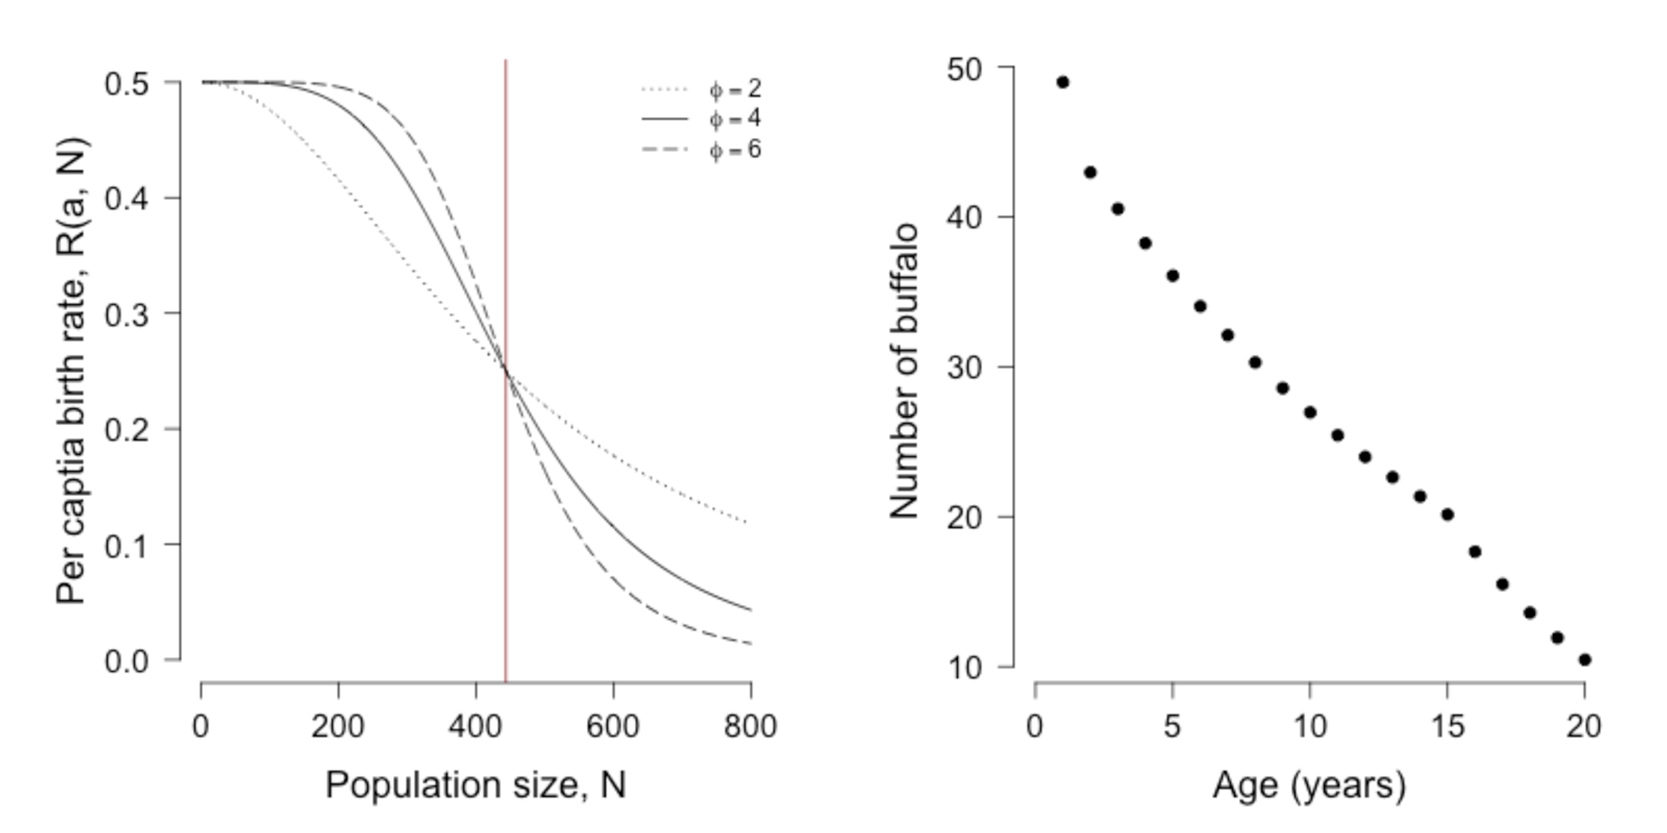
\includegraphics[width = \textwidth]{FigureC1_placeholder.pdf}
  \caption{(left) The per-capita birth rate decreases with increasing population size.  Increasing the abruptness parameter, $\phi$, results in stronger density dependence around, $K$ (red line). (right) (\textbf{NEEDS UPDATED- } The stable age distribution in the absence of infections appears visually similar to field estimates (4, 17)}
  \label{Figure S3.1}
\end{figure}



\begin{table} %hb
\label {Table S3.1.}
\caption{Notation used for model variables and parameters.}
\newcommand{\head}[1]{\textnormal{\textbf{#1}}}
\small
\begin{tabular}{ll} %{12cm}
\hline
\head{Symbol} & \head{Definition}\\
\hline
\textbf{Variables} &   \\
$S(t, a)$ & buffalo susceptible to both infections of age a at time t  \\
$I_T(t, a)$ & buffalo infected with BTB only of age a at time t  \\
$I_B(t, a)$ & buffalo infected with brucellosis only and infectious of age a at time t \\
$I_C(t, a)$ & buffalo co-infected with both pathogens of age a at time t  \\
$R_B(t, a)$ & buffalo persistently infected with brucellosis but no longer infectious of age a at time t  \\
$R_C(t, a)$ & buffalo persistently infected with brucellosis and co-infected with BTB of age a at time t \\
& \\
\textbf{Parameters} &   \\
$b(a)$ & age-specific maximum birth rate at low population size\\
$K $& scaling parameter defining the characteristic population size \\
$\phi $& abruptness parameter controlling the strength of density dependence around K \\ 
$\mu_S(a) $& age-specific mortality rate for susceptible buffalo \\ 
$\mu_T(a) $& age-specific mortality rate for buffalo with BTB only \\ 
$\mu_B(a) $& age-specific mortality rate for buffalo with brucellosis \\ 
$\mu_C$ &age-specific mortality rate for buffalo co-infected with both pathogens \\ 
$\beta_T $ & transmission rate for BTB in susceptible buffalo \\
$\beta_B(a)$ & transmission rate for brucellosis in susceptible buffalo \\
$\beta_{T}^{'}$  & transmission rate for BTB in buffalo with brucellosis \\
$\beta_{B}^{'}$  & transmission rate for brucellosis in buffalo with bTB \\
$\gamma$& recovery rate for brucellosis \\
$\epsilon$& recrudescence rate for brucellosis \\
\hline 
\end{tabular}
\end{table}


\begin{table} %[H]
\label {Table S3.2.}
\caption{Parameter values, dimensions, and references.}
\newcommand{\head}[1]{\textnormal{\textbf{#1}}}
\small
\begin{tabular}{llcc} %{12cm}
\hline
\head{Parameter} & \head{Value} & \head{Dimensions} & \head{Reference}\\*
\hline
$b(a)$ & 0.5 if $a \geq 5$, 0 otherwise & $yr^{-1}$ & - \\*
$K $& 433 & indiv & (16) \\*
$\phi $& 4 & dimensionless & (16)\\* 
$\mu_S(a) $& 0.06 if $2 < a \leq 16$, 0.1 otherwise & $yr^{-1}$ & (16, 29) \\* 
$\mu_T(a) $& $2.82 \mu_S(a)$ & $yr^{-1}$ & Table S2.1 \\* 
$\mu_B(a) $& $3.02 \mu_S(a)$ & $yr^{-1}$ & Table S2.1 \\ 
$\mu_C$ & $8.58 \mu_S(a)$ & $yr^{-1}$ & Table S2.1 \\ 
$\beta_T $ & 0.00013305462 & $indiv^{-1}day^{-1}$ & fit \\
$\beta_B(a)$ & 0.5764065 if $a\geq 5$, ??? otherwise & $day^{-1}$ & fit \\
$\beta_{T}^{'}$  & $\beta_T$ & $indiv^{-1}day^{-1}$ & Table S2.3 \\
$\beta_{B}^{'}$  & $2.09 \beta_{B}(a)$ & $day^{-1}$ & Table S2.3 \\
$\gamma$& 0.5 & $day^{-1}$ & (21)\\
$\epsilon$& 0.3 & $day^{-1}$ & (25, 27, 28) \\
\hline 
\end{tabular}
\end{table} 

\pagebreak

\noindent
These assumptions give the following system of partial differential equations, \\*

\begin{align*}
\Big \{ \frac{\partial}{\partial t} + \frac{\partial}{\partial a} \Big \} S_{}(t, a) &= r(a, N(t)) - (\lambda_{T}(t) + \lambda_{B}(t, a) + \mu_{S}(a)) S(t, a) \\*         
\Big \{ \frac{\partial}{\partial t} + \frac{\partial}{\partial a} \Big \} I_{T}(t, a)&= \lambda_{T}(t) S(t, a) -  (\lambda'_{B}(t, a) - \mu_{T}(a)) I_{T}(t, a) \\*
\Big \{ \frac{\partial}{\partial t} + \frac{\partial}{\partial a} \Big \}  I_{B}(t, a)&=  \lambda_{B}(t, a) S(t, a) - (\lambda'_{T}(t) + \gamma + \mu_{B}(a)) I_{B}(t, a) + \epsilon R_{B}(t, a) \\*
\Big \{ \frac{\partial }{\partial t} + \frac{\partial}{\partial a} \Big \}  I_{C}(t, a)&= \lambda'_{T}(t) I_{B}(t,a) + \lambda'_{B}(t, a) I_{T}(t, a) + \epsilon R_{C}(t, a) - (\gamma + \mu_{C}(a)) I_{C}(t, a) \\*
\Big \{ \frac{\partial}{\partial t} + \frac{\partial}{\partial a} \Big \}  R_{B}(t, a)&=  \gamma I_{B}(t, a) - (\epsilon + \mu_{B}(a)) R_{B}(t, a) \\*            
\Big \{ \frac{\partial}{\partial t} + \frac{\partial}{\partial a} \Big \} R_{C}(t, a)&=  \lambda'_{T} R_{B}(t, a) + \gamma I_{C}(t, a) - (\epsilon + \mu_{C}(a)) R_{C}(t, a) \\* 
\end{align*}

\noindent
with force of infection, \\*

\begin{align*}
\lambda_{T}(t) &= \beta_T \int_{0}^{\infty} (I_t(t,\alpha) + I_{C}(t,\alpha) + R_{C}(t, \alpha)) d\alpha\\*
\lambda'_{T}(t) &= \beta'_T \int_{0}^{\infty} (I_t(t,\alpha) + I_{C}(t,\alpha) + R_{C}(t, \alpha)) d\alpha\\*
\lambda_{B}(t, a) &= \beta_{B}(a) \int_{0}^{\infty} (I_{B}(t,\alpha) + I_{C}(t,\alpha)) d\alpha\\*
\lambda'_{B}(t, a) &= \beta'_{B}(a) \int_{0}^{\infty} (I_{B}(t,\alpha) + I_{C}(t,\alpha)) d\alpha\\*
\end{align*}



\section {Model sensitivity and uncertainty analysis }

We used this model to investigate the consequences of co-infection for Ro and endemic infection prevalence. We calculated Ro numerically using the next generation method (30), reviewed in (31). Additionally, we calculated endemic infection levels of both pathogens before and after the introduction of the co-infecting pathogen. We used Monte Carlo simulation to incorporate uncertainty in the individual-level consequences of co-infection quantified in our data analyses into predictions of Ro and endemic prevalence. Parameter estimates from Cox proportional hazards models are approximately normally distributed with means and standard errors provided in tables S2.1 and S2.2. We drew 1000 random parameter values following the sampling distributions in table S3.3.  For each value, we quantified of Ro and endemic prevalence for both pathogens in populations with and without co-infection.


\pagebreak





\end{document}